\documentclass[tikz,border=10pt]{standalone}
\begin{document}
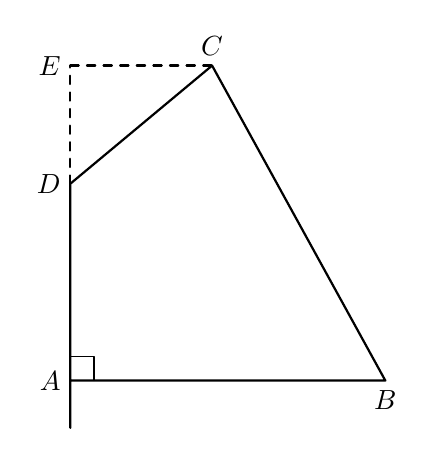
\begin{tikzpicture}[line cap=round,line join=round]
\coordinate (A) at (0,0);
\coordinate (B) at (4,0);
\coordinate (D) at (0,2.5);
\coordinate (E) at (0,4);
\coordinate (C) at (1.8,4);

\draw[thick] (A) -- (B) -- (C) -- (D) -- (0,-0.6);
\draw[dashed,thick] (D) -- (E);
\draw[dashed,thick] (E) -- (C);
\draw (0,0.3) -- (0.3,0.3) -- (0.3,0);

\node[left] at (A) {$A$};
\node[below] at (B) {$B$};
\node[left] at (D) {$D$};
\node[left] at (E) {$E$};
\node[above] at (C) {$C$};
\end{tikzpicture}
\end{document}
